\documentclass[12pt,a4paper,uplatex,dvipdfmx]{jsarticle}
\usepackage{titlesec}
\usepackage{listings,jvlisting}
\usepackage[dvipdfmx]{graphicx}
\usepackage{url}

\usepackage[top=30truemm,bottom=30truemm,left=25truemm,right=25truemm,truedimen]{geometry}

%ここからソースコードの表示に関する設定
\lstset{
  basicstyle={\ttfamily},
  identifierstyle={\small},
  commentstyle={\smallitshape},
  keywordstyle={\small\bfseries},
  ndkeywordstyle={\small},
  stringstyle={\small\ttfamily},
  frame={tb},
  breaklines=true,
  columns=[l]{fullflexible},
  numbers=left,
  xrightmargin=0zw,
  xleftmargin=3zw,
  numberstyle={\scriptsize},
  stepnumber=1,
  numbersep=1zw,
  lineskip=-0.5ex
}
%ここまでソースコードの表示に関する設定
\titleformat*{\section}{\Huge}
\begin{document}
\title{Teller Engineドキュメント}
\author{\texttt{岸 渉憲}}

\maketitle

\section*{はじめに}
TellerEngineはノベルゲーム用のゲームエンジンです。エディターを使用して誰でも気軽にノベルゲームを作れるようになることを目標に開発を進めています。

\section{設計}
\subsection{概要}
できるだけモジュールという単位で機能を切り出せるように設計しています。
TellerEngineは以下の基本的なクラスで構成されています。
\begin{quote}
  \begin{itemize}
    \item TellerCore
    \item Editor 及びその派生クラス
    \item ModuleCore 及びその派生クラス
  \end{itemize}
\end{quote}
\subsection{TellerCore}
TellerCoreは上記のクラス、及びそれ以外のAnimationクラスのなどを管理する中枢となるクラスです。このクラスからModuleCoreの派生クラスであったりEditorクラスを呼び出します。
\subsection{ModuleCore}
モジュールの基底クラス。

\subsubsection{SceneModule}
シーンを構成するモジュールです。具体的には場面やCGシーンなどを移すときに使うことになります。このモジュールをGameModuleにキューとして追加していきます。

\subsection{Editor}
エディターの基底クラス。エディターを編集するクラスは必ずこれを継承する必要があります。

\subsubsection{EpisodeEditor}
csv形式で保存されたシナリオを読み込みEpisodeという単位に分割するためにエディター。

\subsubsection{EpisodeEventEditor}
Episodeファイルにイベントを設定するためのエディター。キャラクターの立ち絵を変更したり入退場させたり背景を変更するイベントを編集・設定できる。

\subsubsection{AssetViewer}
保存したEpisodeファイルやcsvファイルを読み込むためのエディター

\subsection{アーキテクチャ図}
図を簡単にするためEditorクラスがTellerCoreに含まれている図にしているが、実際はEditorクラスを継承したクラス(AssetViewer, EpisodeEditor, EpisodeEventEditor...)が集約されている。
\begin{figure}[tb]
  \centering
  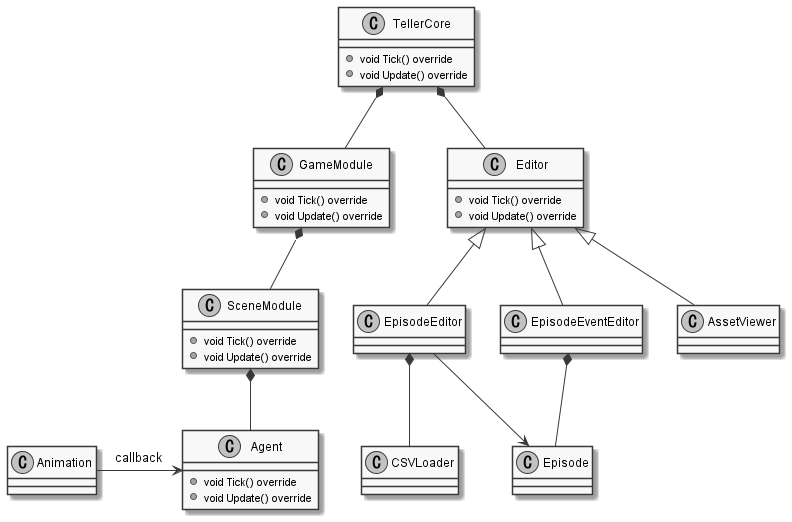
\includegraphics[width=120mm]{architecture.png}
\end{figure}

\newpage
\section{実行環境、製作期間等}
\subsection{実行環境}
以下の環境で動作します。
\begin{quote}
  \begin{itemize}
    \item Windows 10 21H2 build 19044.1706
    \item Visual Studio 2022 Community
    \item 標準C++17
    \item Git
  \end{itemize}
\end{quote}
\subsection{製作期間}
\begin{quote}
  \begin{itemize}
    \item 製作期間 3週間 5/23~6/15日
    \item 製作人数 一人
  \end{itemize}
\end{quote}
Githubリポジトリ
\url{https://github.com/takiren/Teller}

\subsection{その他作品}
Photoshopプラグイン

\url{https://github.com/takiren/ExtendYourPerspectives}

\end{document}